\documentclass[10pt,twocolumn,letterpaper]{article}

\usepackage{cvpr}
\usepackage{times}
\usepackage{epsfig}
\usepackage{graphicx}
\usepackage{amsmath}
\usepackage{amssymb}

% Include other packages here, before hyperref.

% If you comment hyperref and then uncomment it, you should delete
% egpaper.aux before re-running latex.  (Or just hit 'q' on the first latex
% run, let it finish, and you should be clear).
\usepackage[breaklinks=true,bookmarks=false]{hyperref}

\cvprfinalcopy % *** Uncomment this line for the final submission

\def\cvprPaperID{****} % *** Enter the CVPR Paper ID here
\def\httilde{\mbox{\tt\raisebox{-.5ex}{\symbol{126}}}}

% Pages are numbered in submission mode, and unnumbered in camera-ready
%\ifcvprfinal\pagestyle{empty}\fi
\setcounter{page}{1}
\begin{document}

%%%%%%%%% TITLE
\title{Yelp Recommendations}

\author{
Gavriel Adler\\
Carnegie Mellon University\\
{\tt\small gya@andrew.cmu.edu}
% For a paper whose authors are all at the same institution,
% omit the following lines up until the closing ``''.
% Additional authors and addresses can be added with ``\and'',
% just like the second author.
% To save space, use either the email address or home page, not both
\and
Spencer Barton\\
Carnegie Mellon University\\
{\tt\small sebarton@andrew.cmu.edu}
\and
Fridtjof Melle\\
Carnegie Mellon University\\
{\tt\small fmelle@andrew.cmu.edu}
}

\maketitle
%\thispagestyle{empty}

%%%%%%%%% ABSTRACT
\begin{abstract}
   These days when looking for somewhere to eat, people often read online reviews on Yelp. Using machine learning techniques we aimed make this process simpler by giving users specific restaurant recommendations. Reducing their time spent looking through many possible places to eat by offering a specific or small subset of restaurants based on the reviews of similar users, we believe the overall user experience and general profit from using Yelp can be improved and the user should generally have a better chance of succeding in finding a great restaurant for his or her individual taste.

   
\end{abstract}

%%%%%%%%% BODY TEXT
\section{Introduction}

\subsection{The Problem}
Yelp is a popular destination for people looking for a place to eat based on other people's experiences and reviews, gradually becoming a more important factor in their decision-making. While the provided information is quite useful compared to having no information about the restaurant at all, someone looking for a recommendation is bound to the opinions of strangers, who perhaps have very different tastes in food.
\subsection{The Solution}
Our solution is to fix this problem by giving a user personalized recommendations. Based on the user's past reviews, we aim to find a subset of Yelp users with similar taste and predict the scores that the given user would give to restaurants he or she has not yet visited. This allows the person to try a new restaurant with a greater sense of security that he or she will enjoy the experience and not waste money, and would be a nice add-on to the general information provided.
\subsection{Similar work}
The core concept of our pipeline is based on solutions for the 2006-2009 Netflix Prize. This contest was aimed at improving Netflix' algorithm for providing user-specific movie recommendations. It went on over several years with the goal of beating Netflix original recommendation algorithm by a tenth. Although quite extensive algorithms went into the final solutions the general principles has been the inspiration for our solution and we will continue to use papers the contest produced as inspiration for our continued work with the project\cite{KorBell}\cite{BellKor}.

**TODO: Other class project (Fritz)

%=====================================================================

\section{Data Set}

\subsection{Overview}
Yelp holds a massive amount of data to their disposal based on everything that users provide in terms of personal information, business information and everything they put into their reviews. For our purpose Yelp provides a subset of this based on a specific region or city, generated with the same attributes as the real world data, which for our case is Phoenix, Arizona. This provides us with a total of 14303 restaurants and 1.2M reviews, all connected to Phoenix through around 250000 users. The data is originally compiled JSON, which we have expanded to reduce and edit, and then convert to a matrix-based CSV-format for classification and prediction.

\subsection{Users}
In order to generate a user characterizing model we were inclined to extract all the elite users as they contain the most data. Yelp classified 20045 individuals as elite, all with an average of 200 reviews each. In addition we have randomly extracted 2014 sample users not contained within the training data, to test our algorithm on, as well as the top 50 reviewers from the elite users to test the pipeline on. All users are in the same reduced format, only containing the parameters we deem necessary for characterizing the particular users. Below is an example of user-specific data we will use as basis for our models.

\begin{verbatim}
{
    "average_stars": 3.65,
    "name": "Lene",
    "review_count": 214,
    "user_id": "WvhiRlcy-XYwiCof"
}
\end{verbatim}

\subsection{Restaurants}
As Yelp does not limit themselves to restaurants, neither does the original data set. Extracting these was the first part of our extraction. Furthermore, the restaurants contains a lot of information that we wouldn't find particularly interesting for our purposes and subsequently removed attributes as \textit{address}, \textit{hours}, \textit{neighborhoods}, geographical coordinates and general attributes such as \textit{Wi-fi}, \textit{Ambiance}, \textit{Noise level} and \textit{Attire}. We finally end up with a set of 14303 restaurants whereas one example of information we will use is detailed below.

\begin{verbatim}
	{
	    "business_id": "8Jg4S5r79dh",
	    "categories": [
	        "Pizza",
	        "Restaurants"
	    ],
	    "city": "Phoenix",
	    "name": "Mellow Mushroom",
	    "review_count": 62,
	    "average_stars": 3.5,
	    "state": "AZ"
	}
\end{verbatim}

\subsection{Reviews}
While users and restaurants are necessary input information to structure our data and our results, the reviews are the backbone of our predictions and binds all of the data together. With a total of 1.2M reviews we chose to look away from the actual review text, as feature generation through analysis of this would become too significant in our work progress, leaving us with a following structure of our reviews only keeping the provided rating.

\begin{verbatim}
	{
	    "business_id": "HD_D2LTNTL6EXmvH",
	    "review_id": "3vZLrrZ6-kvTO5Q7",
	    "stars": 5,
	    "user_id": "t6GmgDZNeaTnj75NT"
	}
\end{verbatim}

%=====================================================================

\section{Algorithm}

\subsection{Overview}
\begin{figure}[t]
\begin{center}
\fbox{\rule{0pt}{2in}
   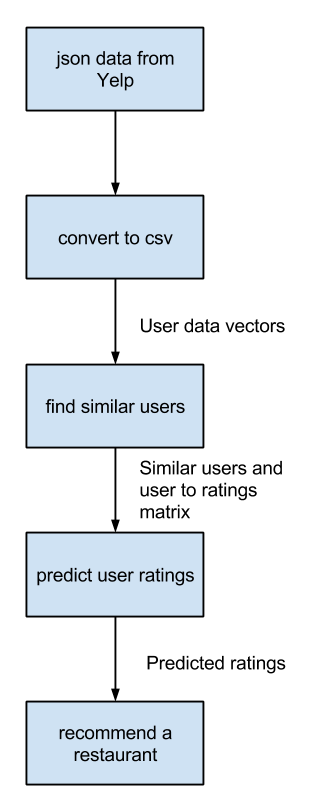
\includegraphics[width=0.3\linewidth]{WorkFlow.png}}
\end{center}
   \caption{A workflow diagram of our pipeline.}
\label{fig:long}
\label{fig:onecol}
\end{figure}

** TODO : Assure most precise description of pipeline given our final algortihm -- does it output an actual restaurant or a MSE for our predictions etc **

Our pipeline takes in a given user, and outputs a restaurant recommendation. In order to do this we first create a feature vector for the person, and find determine the most similar users based on these features. We then see how these similar users rated restaurants the user has not been to, and thus evaluate how the user would rate those restaurants. Finally, the restaurant with the highest expected rating is returned to the user.

\subsection{Parsing the Data and Implementing our models}
In order to perform a proper restaurant predictions and give good recommendations we had to combine all the above data provided in order to map and characterize the users in terms of taste. Mapping users based on their reviews and the general restaurant information is a sizeable, but necessary data operation that was completed through usage of Python's PANDAS module and the NumPy libraries. PANDAS allowed us to read and save .csv files from and to data frames, which, built on top of NumPy arrays, are strictly typed true C arrays and invoke C calls, vastly decreasing run time. To perform PCA and KNN, we used Python's scikit-learn machine learning library. Also built on top of NumPy, it was easy to seamlessly incorporate the library with our existing code. All of the code is visible at \url{https://github.com/sbarton272/PatRec}.

\subsection{User Vectors}
In order to predict the optimal recommendation for a given user, our first step is naturally to describe the user. Using a vector containing a numerical evaluation of the key traits chosen intiuitively keeping everything we found valuable, we can reduce each one to the following parameters:
\begin{verbatim}
	{
	    "user_id": "t6GmgDZNeaTnj75NT",
	    "average_stars": 4.35,
	    "average_price": 2.6,
	   	"mean_diff": 0.5,
	   	"review_count": 9,
	   	"Japanese_num": 2,
	   	"Japanese_star": 3.5,
	   	"Pizza_num": 0,
	   	"Pizza_star": 0,
	   	"American_num": 5,
	   	"American_star": 4,
	   	..
	   	"Bagels_num": 5,
	   	"Bagels_star": 4,
	}
\end{verbatim}

For each user we include general statistics as its average rating, the number of reviews conducted as well as the average price of the restaurants visited, which represents a mean of a normalized price range provided by Yelp for all restaurants which we mapped to the reviews. Furthermore, we included a mean difference between the users rating of each reviewed restaurant compared to the restaurants average rating. 
\\[.5em]
\indent In order to more specifically map the users taste we further included the ratings and visits to each of the different categories classified by Yelp. As each restaurant will be characterized by one or multiple categories within a set array totaling 238 different ones, this maps not only the users interests by which categories he more frequently visits and reviews, but also the average rating of the different types. Although the number of categories is large, each restaurant can as mentioned be characterized by multiple ones providing each user with a sizable set of values, while those not visited are defaulted to zero.

\subsection{Feature selection and dimensionality reduction}
As a next step, we performed dimensionality reduction on the user vectors. We were about to cluster the user vectors to find users who had similar tastes, but most user vectors were very sparse--a user had visited only a handful out of the 238 restaurant categories. In order to reduce the user vector we used PCA and projected the data onto some of the principal components with the highest eigenvalues (how many principal components varied, the trials and results are discussed below). This step inherently weeded out dimensions with low variances which are less useful for identified separated clusters of users, and also had the added bonus of decreasing the run time of the rest of the algorithm. 

\subsection{Finding Similar Users}
** 
TODO: Update for Cross-validated estimation of k when performed

Include results with graphs: Optimal k-Fold Cross-Validation MSE error validating number of similar users to use
**

Our solution creates a feature vector of each user and uses the k Nearest Neighbors algorithm to sort the feature vectors and find k users closest to the person based on the feature vector. To find similar users, we simply run KNN for a single user feature vector on the entire set of user feature vectors, and let the algorithm evaluate the numerically closest ones through a simple distance measure. 

The validation the number of k similar users to keep was done statistically using a K-Fold Cross-Validation Model for K (K=10 partitions I presume??) partitions tracking the MSE inducing for k ranging between 1 and X. 

\subsection{Predicting User Reviews}
In the next step of our pipeline we took in the similar users and their reviews. From the pool of restaurants reviewed by the similar users we predicted a score for each restaurant for a given user using the following weighted average for each restaurant $i$:
\[stars_{i} = w_1 * avg_{usr} + w_2 * avg_{i} + w_3 * similarUserAvg_{i}\]
 where $w_1 + w_2 + w_3 = 1$. $similarUserAvg_i$ was average review for restaurant $i$ from the similar users. Not all similar users would have reviewed the restaurant so this average may have been over as few as 1 to 2 similar users. 
\\[0.5em]
\indent As will be shown below in results the above weighting method did not work well. We were not able to beat the baseline. Therefore we amended the prediction scheme. The basic idea behind prediction is that a rating will likely fall near the restaurant average. Deviation from this average is more likely if there are multiple similar users who liked the restaurant and their ratings are quite different than the restaurant average. Our basic algorithm:
\begin{verbatim}
Per restaurant i
  if similarUsrRatings(i) > V and
      numSimilarUserRating(i) > K
    prediction = w1*userAvg
                 +w2*similarUsrAvg(i)
                 +w3*resturantAvg(i)
  else
    prediction = .5*userAvg +
                 .5*resturantAvg(i)
\end{verbatim}

\subsection{Recommendation}
The final step is to recommend a restaurant based on the predicted ratings. We simply recommend the highest predicted rated restaurant.

\subsection{Validating Results}
While our algorithm outputs a restaurant recommendation it is tough to validate based upon a single recommendation since a baseline cannot be easily established. The issue is that we do not have a way to provide real users our recommendation and see how well they like the recommendation. However, validating our rating prediction is simpler because we can compare to the actual ratings that users gave to restaurants. While we are able to predict on the restaurant rating we are not able to validate the actual choice of recommended restaurants.
\\[0.5em]
\indent Our validation process is to run our algorithm with a training set of users and reviews and then predict previously known ratings for users from a testing set. Because our system predicts ratings for only restaurants visited by the similar users, there are usually more predicted ratings than actual reviews. Therefore we take the intersection of the predicted ratings and the actual ratings and use this set to calculate our error.

%=====================================================================

\section{Results}

\subsection{Overview}
Overall we did not beat the baseline. Over a range of KNN and PCA parameters we were not able to beat our baseline.

Why not? Be believe that our results show that a given user's review is generally closer to the restaurant average rather than the similar user's average rating. Basically our the premise that similar users' preferences are a proxy for a users' preferences does not seem to be valid.

- Number changed over baseline
- 

- Did not beat baseline
- Why not?
- baseline is too similar to our prediction model
- Similar users don't really have enough effect
- You are closer to the avg than you are to the avg similar users

- PCA: Overfitting too close, then MSE spike and drop (stop overfitting)
- KNN eventually have too many similar users

\subsection{Parameters}
Our basic model relied on five input parameters:

\begin{enumerate}
\item The $K_{KNN}$ for KNN
\item The number of principal components the user vector was projected onto, $P$
\item Three weights applied to our three parameters used to make a prediction: 
\begin{enumerate}
\item $w_{u}$, the weight given to the user's average review score
\item $w_{s}$, the weight given to how a user's $K_{KNN}$ similar users rated the restaurant in question
\item $w_{r}$, the weight given to the restaurant's average review score
\end{enumerate}
\end{enumerate}
We tried a range of $K_{KNN}$ and $P$ values to find the best and then selected weights based upon intuition. For the three weights, we used $w_{u}=.33$, $w_{s}=.33$, and $w_{r}=.33$, evenly weighting all three factors.

\subsection{Baseline}

For our baseline, we used $w_{u}=.5$, $w_{s}=0$, and $w_{r}=.5$. Our goal was to see how our algorithm would perform without any knowledge of similar users, so we kept $w_{u}$ and $w_{r}$ weighted evenly, but removed $w_{s}$ entirely.

\subsection{Parameter Tuning}

%=====================================================================

\section{Challenges}

\begin{figure}[t]
\begin{center}
\fbox{\rule{0pt}{2in}
   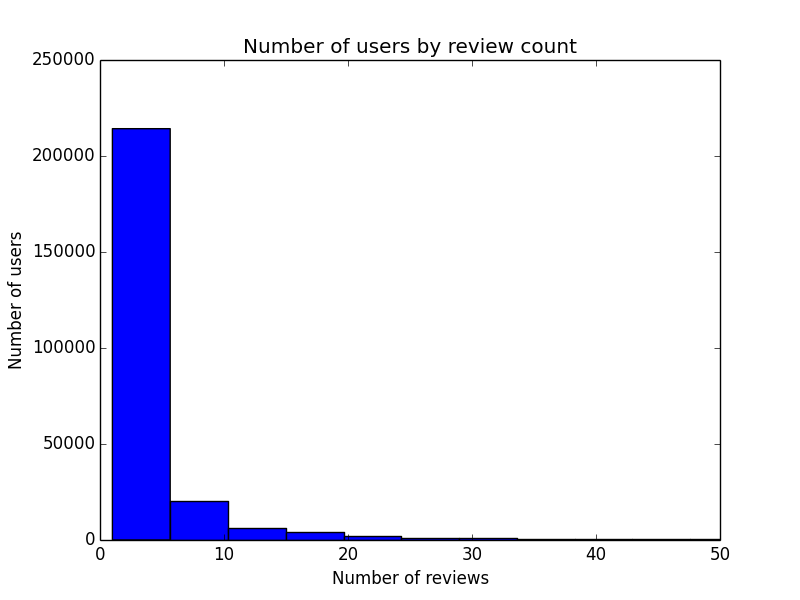
\includegraphics[width=0.9\linewidth]{usrCnt.png}}
\end{center}
   \caption{A histogram of the number of users organized by review count.}
\label{fig:usrCnt}
\end{figure}

\begin{figure}[t]
\begin{center}
\fbox{\rule{0pt}{2in}
   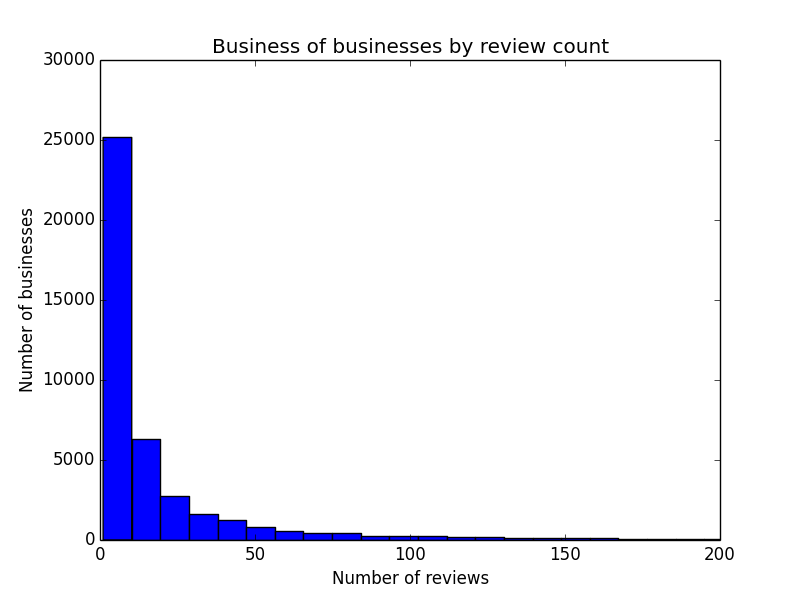
\includegraphics[width=0.9\linewidth]{bizCnt.png}}
\end{center}
   \caption{A histogram of the number of businesses organized by review count.}
\label{fig:bizCnt}
\end{figure}

\subsection{Review Sparsity}
One of our base assumptions is that users and establishments have enough reviews for us to extrapolate future reviews. However we may be pushing this limit. As can be seen in Figure~\ref{fig:usrCnt} a substantial majority of users, $85\%$, have five or fewer reviews. Since reviews likely provide the best information on user tastes we will likely have trouble classifying users by reviews alone. Likewise establishments also have a small number of reviews which will make it hard to predict potential ratings. However this is not quite as much of a problem as the user data. As can be seen in Figure~\ref{fig:bizCnt}, the majority, $60\%$, of businesses have fever than ten reviews.

\subsection{Data Cleanliness}
We have encountered issues with duplicate reviews as well as establishments not from the Phoenix area. Both are removed from our data set.

%=====================================================================

\section{Future work}

\subsection{Evaluation of classifier: Generative models}
Our current classifier, the KNN, is of the Deterministic Association type, making no assumptions of data distribution or correlation of any kind. This leaves a big room of improvement as our data contains unused information that we can take into equation. Rather than just sorting users based on numerical values in a deterministic manner, can further cluster and develop user-characterizing models based on taste. This edge especially relates to the fact that every restaurant is characterized by a set of labels such as \textit{Mexican}, \textit{Pizza}, \textit{American} among others that permits us to map a users taste based on general visitation and following reviews. Not only can this play a part in the development of similarity, but also help further weight the restaurant valuations and predictions in the following evaluation. We currently imagine using techniques such as Naïve Bayes with possible follow-up by a GMM variation.

\subsection{Geographic Restrictions}
As mentioned our extracted data set contains users, restaurants and reviews are somehow related to Phoenix, AZ. Although, this does not mean that every user, restaurant or review is directly connected to this region. If a user has done one review of one restaurant in Phoenix, all his other reviews and effectively the corresponding restaurants is included in the data set. For now we have looked away from geographical locations, in order to have our algorithm give the best possible recommendation regardless of its location, but this is something that would be interesting to give more attention on a next iteration.

\subsection{Discovery}
Spotify and other music services provide an option for users to explore music outside of their current preferences or to add diversity. This project may be more useful to Yelp as a feature that provides a unique recommendation. Our algorithm is biased towards recommending similar restaurants which may not be what users are actually looking for when they ask for a recommendation.

%=====================================================================

%uncomment and add \cite{}'s for bilbiography. fill in egbib.bib file
{\small
\bibliography{egbib}
\bibliographystyle{plain}}

\end{document}
